\documentclass[landscape,a0,final]{a0poster}
\usepackage[dvipsnames,svgnames]{xcolor}
\usepackage{tikzposter} % here most of the things are defined
% change parameters only after this line You can also start a new column with an arbitrary 
% x-coordinate by specifying explicitly the coordinate of the new block node as follows:
\usepackage[czech]{babel}
\usepackage[utf8]{inputenc}
\usepackage{wrapfig}
\usepackage{url}

%Used for better control on code display

\usepackage[margin=\margin cm, paperwidth=197cm, paperheight=100cm]{geometry}

% \setbackgrounddarkcolor{ForestGreen!70!black}
% \setbackgroundlightcolor{YellowGreen!90!}

% \setfirstcolor{YellowGreen!80!}
% \setsecondcolor{gray!80!}
% \setthirdcolor{red!80!black}

\title{Improving the Apollo 12 landing site mapping\\with Chandrayaan $M^3$ data}
\author{Yann Chemin$^{1,2}$, Ian Crawford$^1$, Roberto Bugiolacchi$^1$, Huma Irfan$^1$ and Louise Alexander$^1$\\
$^1$Birkbeck College, University of London, U.K. ~ $^2$IWMI, Pelawatte, Sri Lanka}

\usetemplate{1}
\setinstituteshift{1}

\setblocktitleheight{2}
\setblockspacing{1}

\begin{document}
\ClearShipoutPicture
\AddToShipoutPicture{\BackgroundPicture}
\noindent
\tikzstyle{every picture}+=[remember picture]
\begin{tikzpicture}
\initializesizeandshifts
\titleblock{90}{1}
% \setblocktitleheight{1}

%\addlogo[north west]{(2,-1)}{9cm}{./svg_images/Grass_GIS.pdf}
%\addlogo[north east]{(-2,-2.5)}{11cm}{./svg_images/IWMI_logo.pdf}

%%%%%%%%%%%%%%%%%%%%%%%%%%%%%%%%%%%%%%%%%%%%%%%%%%%%%%%%%%%%%%%%%%%%%%%%%%%%%%%%
\blocknode{Abstract}{
\small \noindent The geology of the Apollo 12 landing site has been the subject of many studies, including recently by Korotev et al. (2011) and Snape et al. (2013). This research attempts to bring additional understanding from a remote sensing perspective using the Moon Mineralogy Mapper ($M^3$) sensor data, onboard the Chandrayaan lunar orbiter. This has a higher spatial-spectral resolution sensor than the Clementine UV-Vis sensor and provides the opportunity to study the lunar surface with detailed spectral signatures.\newline

Mapping of FeO (wt\%) and TiO 2 (wt\%) is done using the methods of Lucey et al. (2000) and Wilcox et
al. (2005). A FeO \& TiO 2 processing module (i.feotio2) is made specifically for this research within the Free \& Open Source Software GRASS GIS (Neteler et al., 2012). Attempts will be made to estimate the lava flow thickness using the method of Bugiolacchi et al. (2006) and individual lava layers thicknesses (Weider et al., 2010). Integration of this new information will be put in perspective and integrated with previous work. Analysis from the combined higher spatial and spectral resolutions will improve the accuracy of the geological mapping at the Apollo 12 landing site.\newline
}


%%%%%%%%%%%%%%%%%%%%%%%%%%%%%%%%%%%%%%%%%%%%%%%%%%%%%%%%%%%%%%%%%%%%%%%%%%%%%%%%
\blocknode{Previous interpretations}{
Korotev et al. (2011) reviewed the lunar research done until recently, with a special interest in the Apollo 12 landing site and its vicinity. Among the information newly deducted, are a geological context block diagram 1 (Figure below) along with an Apollo 12 landing site interpretive cross-section. Fortezzo and Hare (2013) completed the digital renovation of the 1:5,000,000 lunar geological maps series, enhanced with LOLA-LRO information.\newline
\begin{center}
	\begin{tabular}{cc}
		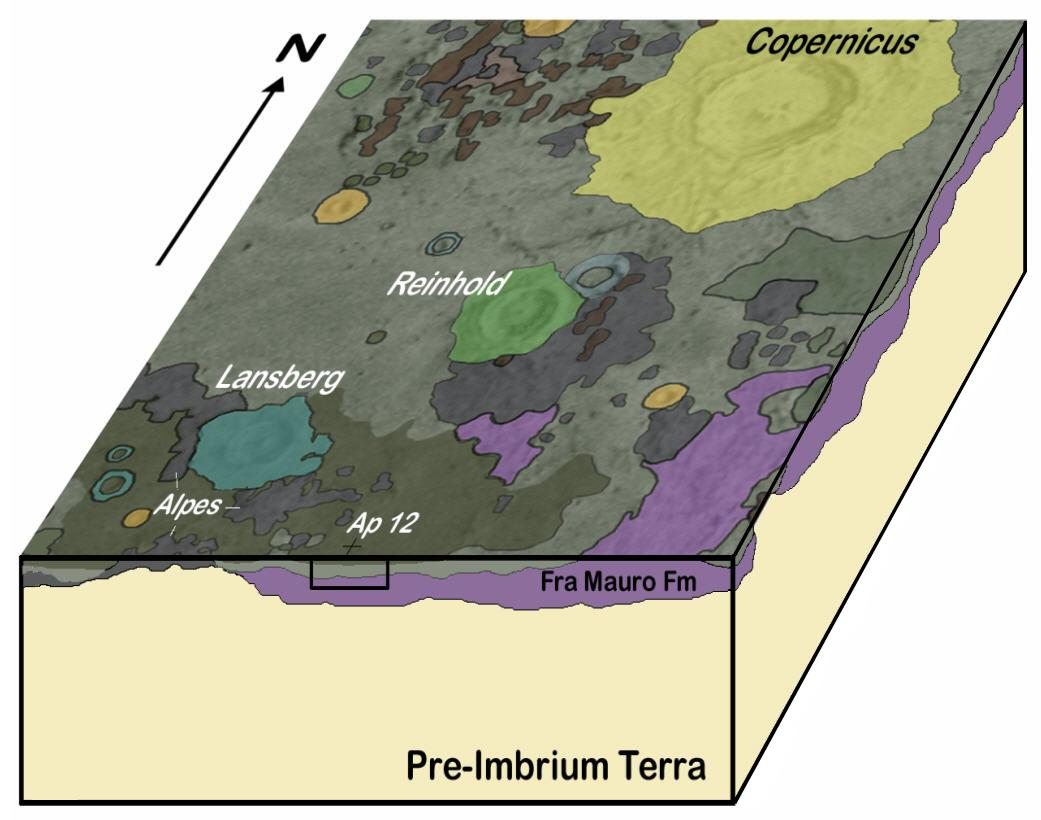
\includegraphics[width=0.45\textwidth]{./images/Korotev_block}
		&
		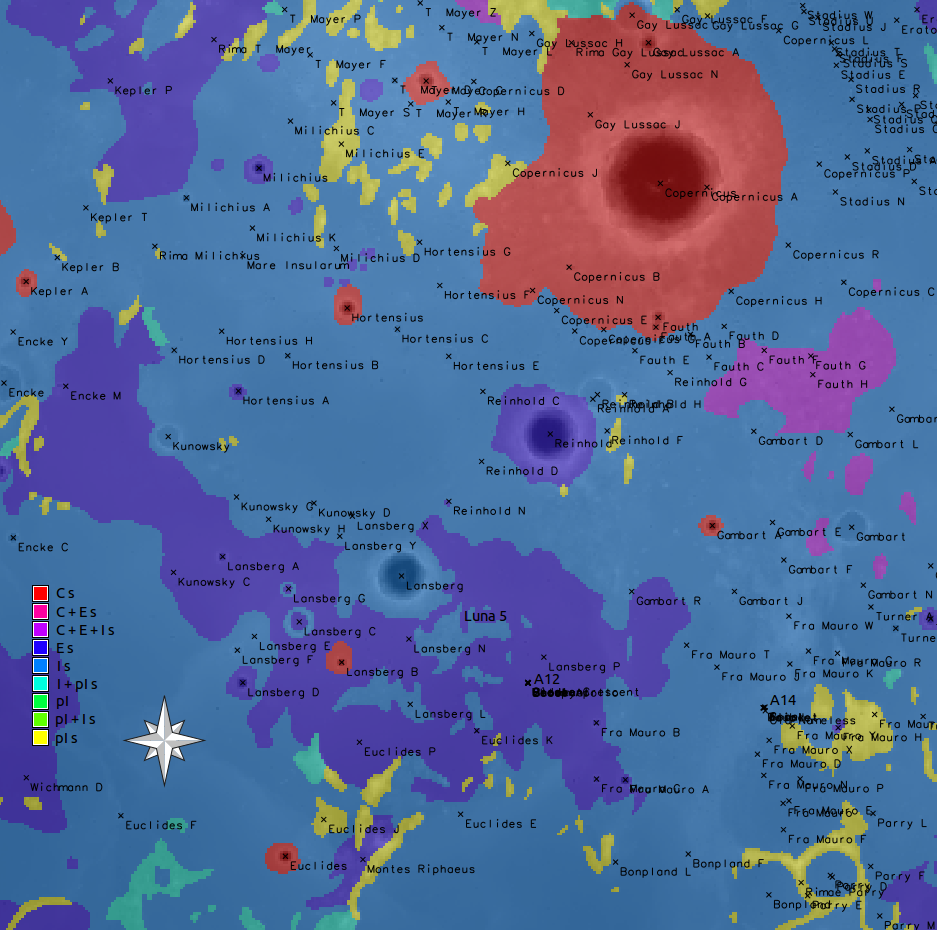
\includegraphics[width=0.45\textwidth]{./images/A12region}
	\end{tabular}\newline
Figure 2: a) Korotev et al (2011) geological block of Apollo 12 landing site\\
b)  Fortezzo and Hare (2013) geological maps series with moon nomenclature.
\end{center}
}


%%%%%%%%%%%%%%%%%%%%%%%%%%%%%%%%%%%%%%%%%%%%%%%%%%%%%%%%%%%%%%%%%%%%%%%%%%%%%%%%
\getcurrentrow{box}
\coordinate (funkcionalita) at (box.south west);
\coordinate (funkcionalitaeast) at (box.east);
\coordinate (screenshot) at (box.north west);

\blocknodew[($(funkcionalita)+(20,-1)$)]{35}{References}{
\scriptsize
\begin{flushleft}
\begin{tabular}{rp{0.9\textwidth}}
Bugiolacchi et al. (2006) &  Planetary Science. 41(2):285-304.\\{}
Fortezzo et al. (2013) & LPI Contributions, 1719:2114.\\{}
Korotev et al. (2011) & Geochimica et Cosmochimica Acta. 75(6):1540-1573.\\{}
Lucey et al. (2000) & J. Geophys. Res. 105(E8): 20297-20305.\\{}
Neteler et al. (2012) & Environment \& Modeling Software, 31:124-130.\\{}
Snape et al. (2013) & LPSC Abstracts 44:1044.\\{}
Weider et al. (2010) & Icarus, 209, 323-336.\\{}
Wilcox et al. (2005) & J. Geophys. Res. 110(E11):2156-2202.\\{}
\end{tabular}
\end{flushleft}
\smallskip
\hrulefill
\vspace{-5pt}

\begin{center}
\begin{tabular}{cp{0.9\textwidth}}
\begin{minipage}{0.15\textwidth}

\includegraphics[width=0.7in]{./images/grass_qr.pdf}
\end{minipage}

\begin{minipage}{0.3\textwidth}
\small {\url{www.bbk.ac.uk}}
\end{minipage}

\begin{minipage}{0.15\textwidth}

\includegraphics[width=0.7in]{./images/grass_qr.pdf}
\end{minipage}

\begin{minipage}{0.3\textwidth}
\small {\url{grass.osgeo.org}}
\end{minipage}
\end{tabular}
\end{center}

\hrulefill
\vspace{14pt}
\begin{center}
\newcommand{\logowidth}{5em}
\newcommand{\logospace}{\hspace{0.1em}}
\noindent

\includegraphics[width=\logowidth]{./svg_images/public_domain_logo.pdf}
%\raisebox{0.7\height}{\logospace 2013 GRASS Development Team}
\end{center}
}

\startsecondcolumn
%%%%%%%%%%%%%%%%%%%%%%%%%%%%%%%%%%%%%%%%%%%%%%%%%%%%%%%%%%%%%%%%%%%%%%%%%%%%%%%%
\blocknode{Clementine data}{
\smallskip

\begin{center}
 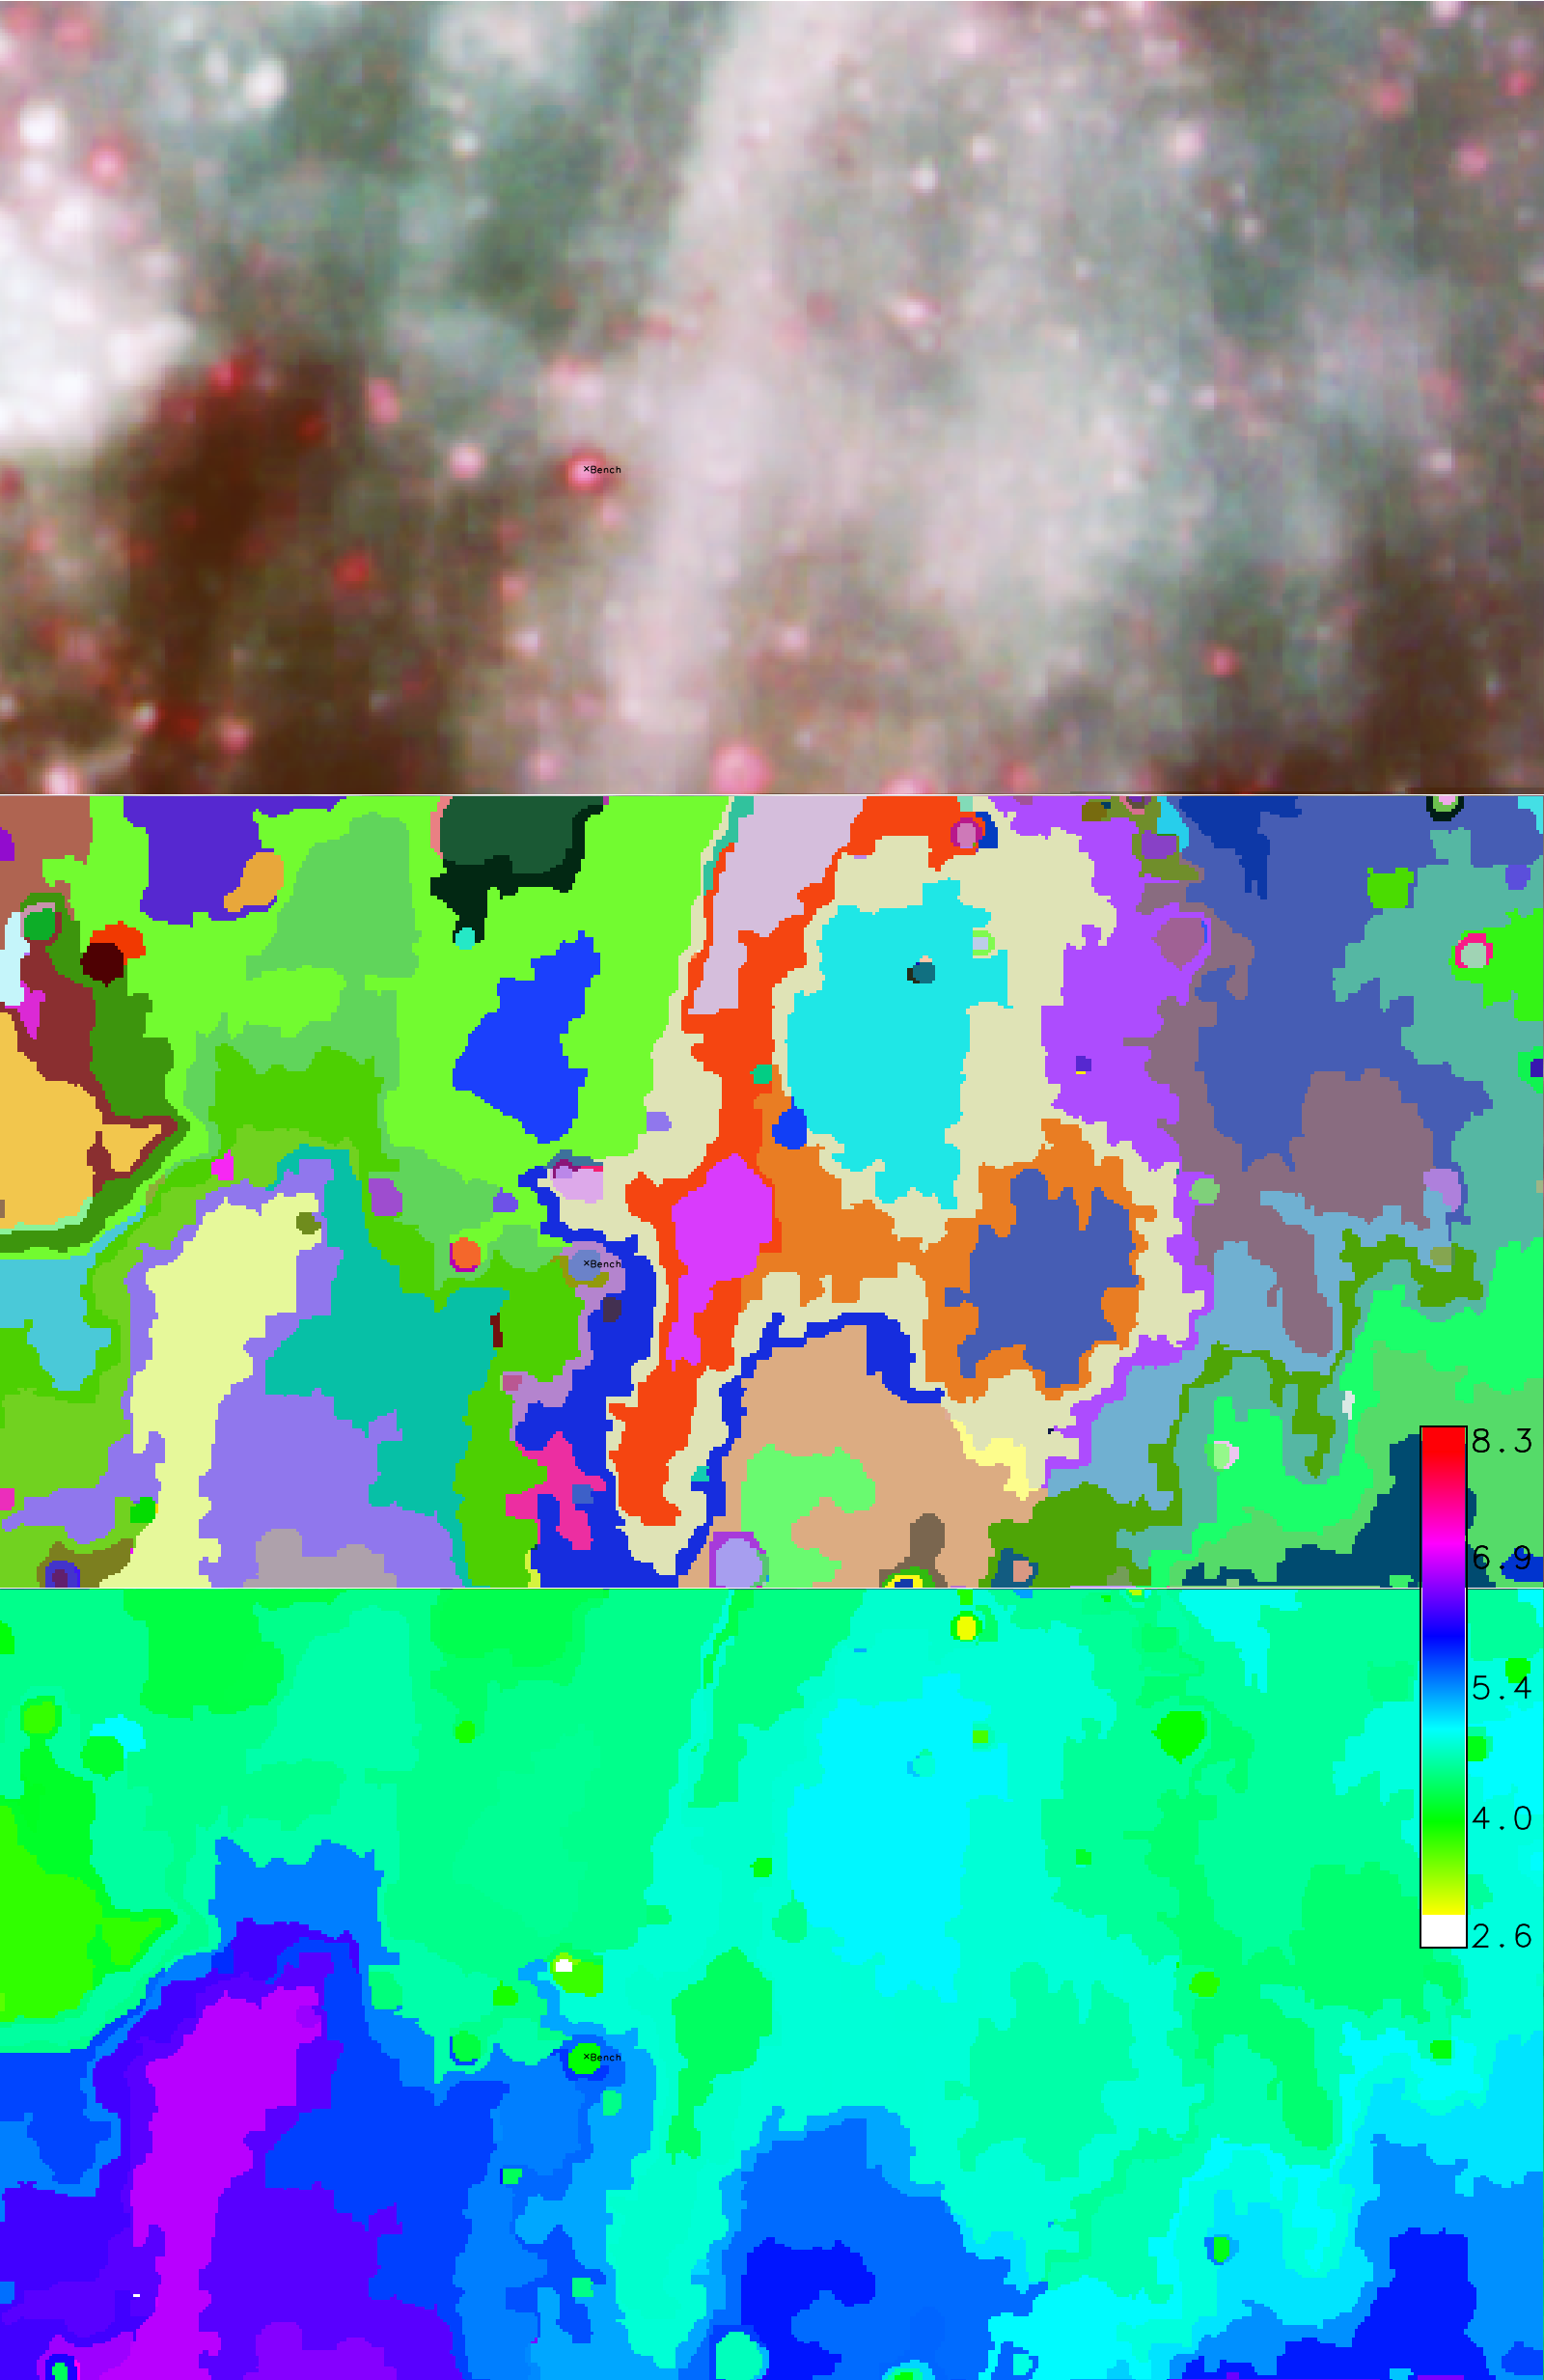
\includegraphics[width=0.75\textwidth]{./images/Clementine}
 \newline
 Figure 1: Clementine RGB153, segmentation and FeO (wt\%) per segmentation class.
\end{center}
}



\startthirdcolumn
%%%%%%%%%%%%%%%%%%%%%%%%%%%%%%%%%%%%%%%%%%%%%%%%%%%%%%%%%%%%%%%%%%%%%%%%%%%%%%%%
\blocknode{$M^3$ data analysis}{
nn
\newline

\begin{center}
 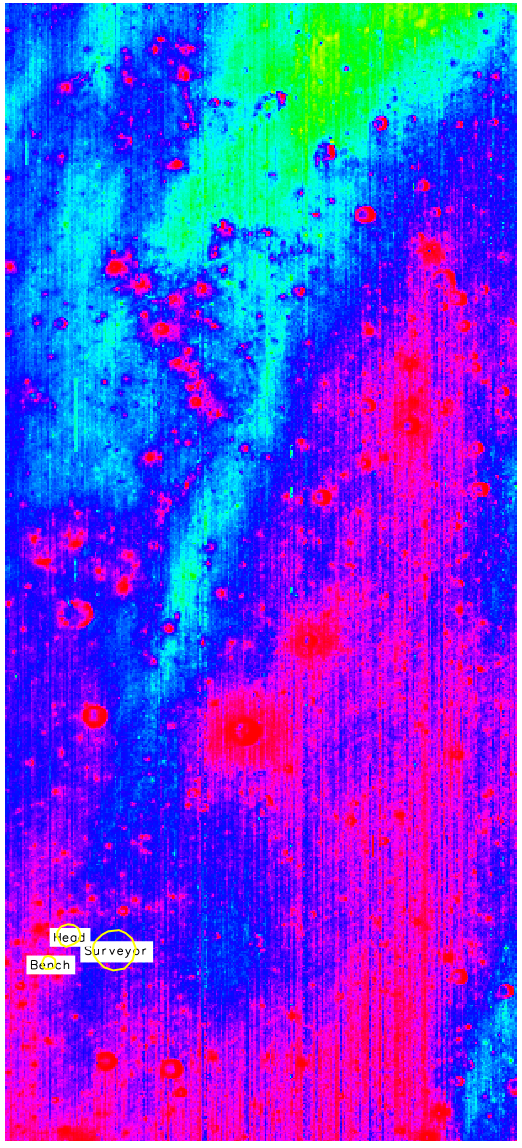
\includegraphics[width=0.5\textwidth]{./images/M3FEOlarge}
 \newline
 Figure 3: FeO
\end{center}

}





\startfourthcolumn

%%%%%%%%%%%%%%%%%%%%%%%%%%%%%%%%%%%%%%%%%%%%%%%%%%%%%%%%%%%%%%%%%%%%%%%%%%%%%%%%
\blocknode{Segmentation of PCA elements}{
GRASS GIS segmentation of the PCA of the full temporal archive of MODIS EVI.
\newline

A summary of the code needed to reach this point of analysis is here.\newline
\hrule
{\footnotesize \fontfamily{pcr}\selectfont i.group \textcolor{blue}{group}=pca\_group \textcolor{blue}{input}=\$(g.mlist \textcolor{blue}{type}=rast \textcolor{blue}{pattern}=*h28v07*EVI)\newline
i.pca \textcolor{blue}{input}=pca\_group \textcolor{blue}{output\_prefix}=pca\_ \textcolor{blue}{percent}=99 --o\newline
\#Here, run {\it i.group} interactively to add the PCA output files you want to use for segmentation\newline
i.segment \textcolor{blue}{group}=seg\_group \textcolor{blue}{output}=seg \textcolor{blue}{threshold}=0.9 \textcolor{blue}{memory}=3000 \textcolor{blue}{iterations}=100 --o\newline}
\hrule
}


%%%%%%%%%%%%%%%%%%%%%%%%%%%%%%%%%%%%%%%%%%%%%%%%%%%%%%%%%%%%%%%%%%%%%%%%%%%%%%%%
\blocknode{Temporal PCA-based classification}{
Classes found to follow one crop per year
\newline

\begin{center}
 
\includegraphics[width=0.55\textwidth]{./images/startup_banner_isis}\newline
 \newline
 Figure 4: Single-crop classes from PCA.
\end{center}

}


\end{tikzpicture}

\end{document}
